\documentclass{beamer}
\usetheme{Madrid}

\title{CONTROL SYSTEMS}
\author{Rishitha.N\\EE18BTECH11033}
\centering
\date{GATE 2016 Q19(EC SECTION)}
\usepackage[document]{ragged2e}
\begin{document}
\maketitle
\begin{frame}{QUESTION}
The response of the system
\begin{equation}
            G(s)= \frac{s-2}{(s+1)(s+3)} ,
 \end{equation} 
to the unit step input u(t) is y(t). The value of \(\frac{dy}{dt}\) at t=0^+ is:
\end{frame}
\begin{frame}{SOLUTION}
Input of the system,
\begin{equation}
     x(t) = u(t) 
\end{equation}
 Where u(t) is a unit step input.
 The Laplace transform x(t) is:
 \begin{equation}
     X(s) =  \int_{-\infty}^{\infty}x(t) e^{-st} dt
 \end{equation}
 Therefore,
 \begin{equation}
     X(s) =  \frac{1}{s}
 \end{equation}

\end{frame}
\begin{frame}{Solution}
  \begin{itemize}
We know that, 
\begin{equation}
  Y(s) = X(s)H(s)
\end{equation}
in Laplace domain.So,
\begin{equation}
Y(s) = \frac{s-2}{s(s+1)(s+3)}
\end{equation}
By doing partial fractions,
\begin{equation}
    \frac{s-2}{s(s+1)(s+3)} = \frac{A}{s} + \frac{B}{s+1} + \frac{C}{s+3} 
\end{equation}
\end{itemize}

\end{frame}

\begin{frame}{SOLUTION}
  
 On solving,
\begin{equation}
A = \frac{-2}{3} , B = \frac{3}{2} , C= \frac{-5}{6}
\end{equation}
From this,
\begin{equation}
    Y(s) = \frac{-2}{3s} + \frac{3}{2(s+1)} + \frac{-5}{6(s+3}
\end{equation}
The inverse Laplace transform of Y(s) is:
\begin{equation}
        y(t) = (\frac{-2}{3}+\frac{3}{2}e^-^t + \frac{-5}{6}e^-^3^t)u(t)
\end{equation}
On differentiating we get,
\begin{equation}
    \frac{dy(t)}{dt} = \frac{-3}{2}e^-^t + \frac{5}{2}e^-^3^t
\end{equation}
Therefore,
 \begin{equation}
    \frac{dy(0^+)}{dt} = \frac{-3}{2} + \frac{5}{2} = 1
\end{equation}


 
\end{frame}

\begin{frame}


   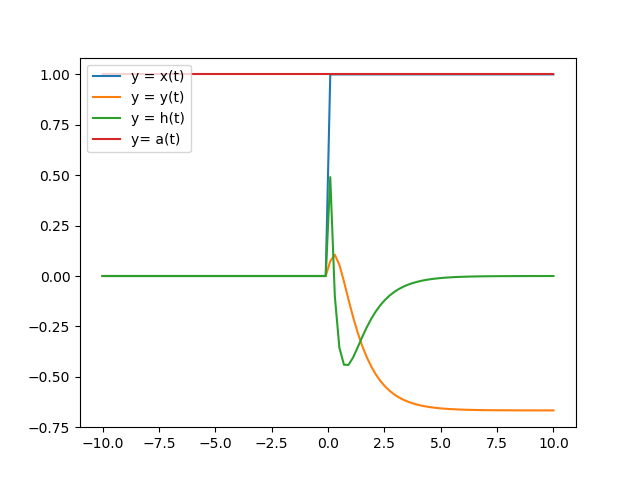
\includegraphics[scale = 0.7]{Graph.png}
    

\end{frame}

\end{document}
